%!TEX TS-program = xelatex

% Шаблон документа LaTeX создан в 2018 году
% Алексеем Подчезерцевым
% В качестве исходных использованы шаблоны
% 	Данилом Фёдоровых (danil@fedorovykh.ru) 
%		https://www.writelatex.com/coursera/latex/5.2.2
%	LaTeX-шаблон для русской кандидатской диссертации и её автореферата.
%		https://github.com/AndreyAkinshin/Russian-Phd-LaTeX-Dissertation-Template

\documentclass[a4paper,14pt]{article}


%%% Работа с русским языком
\usepackage[english,russian]{babel}   %% загружает пакет многоязыковой вёрстки
\usepackage{fontspec}      %% подготавливает загрузку шрифтов Open Type, True Type и др.
\defaultfontfeatures{Ligatures={TeX},Renderer=Basic}  %% свойства шрифтов по умолчанию
\setmainfont[Ligatures={TeX,Historic}]{Times New Roman} %% задаёт основной шрифт документа
\setsansfont{Comic Sans MS}                    %% задаёт шрифт без засечек
\setmonofont{Courier New}
\usepackage{indentfirst}
\frenchspacing

\renewcommand{\epsilon}{\ensuremath{\varepsilon}}
\renewcommand{\phi}{\ensuremath{\varphi}}
\renewcommand{\kappa}{\ensuremath{\varkappa}}
\renewcommand{\le}{\ensuremath{\leqslant}}
\renewcommand{\leq}{\ensuremath{\leqslant}}
\renewcommand{\ge}{\ensuremath{\geqslant}}
\renewcommand{\geq}{\ensuremath{\geqslant}}
\renewcommand{\emptyset}{\varnothing}

%%% Дополнительная работа с математикой
\usepackage{amsmath,amsfonts,amssymb,amsthm,mathtools} % AMS
\usepackage{icomma} % "Умная" запятая: $0,2$ --- число, $0, 2$ --- перечисление

%% Номера формул
%\mathtoolsset{showonlyrefs=true} % Показывать номера только у тех формул, на которые есть \eqref{} в тексте.
%\usepackage{leqno} % Нумерация формул слева	

%% Перенос знаков в формулах (по Львовскому)
\newcommand*{\hm}[1]{#1\nobreak\discretionary{}
	{\hbox{$\mathsurround=0pt #1$}}{}}

%%% Работа с картинками
\usepackage{graphicx}  % Для вставки рисунков
\graphicspath{{images/}}  % папки с картинками
\setlength\fboxsep{3pt} % Отступ рамки \fbox{} от рисунка
\setlength\fboxrule{1pt} % Толщина линий рамки \fbox{}
\usepackage{wrapfig} % Обтекание рисунков текстом

%%% Работа с таблицами
\usepackage{array,tabularx,tabulary,booktabs} % Дополнительная работа с таблицами
\usepackage{longtable}  % Длинные таблицы
\usepackage{multirow} % Слияние строк в таблице
\usepackage{float}% http://ctan.org/pkg/float

%%% Программирование
\usepackage{etoolbox} % логические операторы


%%% Страница
\usepackage{extsizes} % Возможность сделать 14-й шрифт
\usepackage{geometry} % Простой способ задавать поля
\geometry{top=20mm}
\geometry{bottom=20mm}
\geometry{left=20mm}
\geometry{right=10mm}
%
%\usepackage{fancyhdr} % Колонтитулы
% 	\pagestyle{fancy}
%\renewcommand{\headrulewidth}{0pt}  % Толщина линейки, отчеркивающей верхний колонтитул
% 	\lfoot{Нижний левый}
% 	\rfoot{Нижний правый}
% 	\rhead{Верхний правый}
% 	\chead{Верхний в центре}
% 	\lhead{Верхний левый}
%	\cfoot{Нижний в центре} % По умолчанию здесь номер страницы

\usepackage{setspace} % Интерлиньяж
\onehalfspacing % Интерлиньяж 1.5
%\doublespacing % Интерлиньяж 2
%\singlespacing % Интерлиньяж 1

\usepackage{lastpage} % Узнать, сколько всего страниц в документе.

\usepackage{soul} % Модификаторы начертания

\usepackage{hyperref}
\usepackage[usenames,dvipsnames,svgnames,table,rgb]{xcolor}
\hypersetup{				% Гиперссылки
	unicode=true,           % русские буквы в раздела PDF
	pdftitle={Заголовок},   % Заголовок
	pdfauthor={Автор},      % Автор
	pdfsubject={Тема},      % Тема
	pdfcreator={Создатель}, % Создатель
	pdfproducer={Производитель}, % Производитель
	pdfkeywords={keyword1} {key2} {key3}, % Ключевые слова
	colorlinks=true,       	% false: ссылки в рамках; true: цветные ссылки
	linkcolor=black,          % внутренние ссылки
	citecolor=black,        % на библиографию
	filecolor=magenta,      % на файлы
	urlcolor=black           % на URL
}
\makeatletter 
\def\@biblabel#1{#1. } 
\makeatother
\usepackage{cite} % Работа с библиографией
%\usepackage[superscript]{cite} % Ссылки в верхних индексах
%\usepackage[nocompress]{cite} % 
\usepackage{csquotes} % Еще инструменты для ссылок

\usepackage{multicol} % Несколько колонок

\usepackage{tikz} % Работа с графикой
\usepackage{pgfplots}
\usepackage{pgfplotstable}

% ГОСТ заголовки
\usepackage[font=small]{caption}
%\captionsetup[table]{justification=centering, labelsep = newline} % Таблицы по правобу краю
%\captionsetup[figure]{justification=centering} % Картинки по центру


\newcommand{\tablecaption}[1]{\addtocounter{table}{1}\small \begin{flushright}\tablename \ \thetable\end{flushright}%	
\begin{center}#1\end{center}}

\newcommand{\imref}[1]{рис.~\ref{#1}}

\usepackage{multirow}
\usepackage{spreadtab}
\newcolumntype{K}[1]{@{}>{\centering\arraybackslash}p{#1cm}@{}}


\usepackage{xparse}
\usepackage{fancyvrb}

\RecustomVerbatimCommand{\VerbatimInput}{VerbatimInput}
{
	fontsize=\footnotesize    
}

\usepackage{tocloft}
\renewcommand{\cftsecleader}{\cftdotfill{\cftdotsep}}
\begin{document} % конец преамбулы, начало документа
	\begin{titlepage}
	\begin{center}
 		ФЕДЕРАЛЬНОЕ  ГОСУДАРСТВЕННОЕ АВТОНОМНОЕ \\
		ОБРАЗОВАТЕЛЬНОЕ УЧРЕЖДЕНИЕ ВЫСШЕГО ОБРАЗОВАНИЯ\\
		«НАЦИОНАЛЬНЫЙ ИССЛЕДОВАТЕЛЬСКИЙ УНИВЕРСИТЕТ\\
		«ВЫСШАЯ ШКОЛА ЭКОНОМИКИ»
	\end{center}
	
	\begin{center}
		\textbf{Московский институт электроники и математики}
		
		\textbf{им. А.Н.Тихонова НИУ ВШЭ}
		
		\vspace{2ex}
		
		\textbf{Департамент компьютерной инженерии}
	\end{center}
	\vspace{1ex}	
	
	\begin{center}
	\textbf{ОТЧЕТ\\
		ПО ЛАБОРАТОРНОЙ РАБОТЕ №6
	}
	\end{center}	
	\vspace{2ex}
	\begin{center}
		по дисциплине «Проектирование систем на кристалле»
	\end{center}	

	\vspace{2ex}

	\begin{flushright}
		\textbf{Выполнили:}
		
		\vspace{2ex}
		
		Студенты группы БИВ174
		
		Бригада №5
		
		\vspace{2ex}
		
		Подчезерцев Алексей Евгеньевич
		
		Солодянкин Андрей Александрович
		\vspace{2ex}
		
	\end{flushright}

	\vfill
	\begin{center}
		Москва \the\year \, г.
	\end{center}
	
\end{titlepage}
\addtocounter{page}{1}
	\tableofcontents
	\pagebreak
	\section{Задание}
	
	\begin{enumerate}
		\item Разработайте RТL-модель и тест для рассмотренного счетчика . При возникновении
		сложностей обратитесь к дополнительным материалам к данной главе. Сравните полученные
		результаты.
		
		\item Проведите симуляцию модуля clk\_div, файлы с описанием которого находятся в
		дополнительных материалах к данной практической работе. Определите частоту выходного
		сигнала clk\_out. Измените код так, чтобы скважность сигнала составляла 20 %, 50 %. Опишите
		полученные результаты.
		
		\item Проанализируйте работу модуля pwm из дополнительных материалов к данной практической
		работе . Определите, в каких случаях светодиод будет светить ярче. Определите скважность
		выходного сигнала pwm\_out для каждого случая. Проанализируйте временные диаграммы на
		Рисунке 6.12. Разработайте собственный модуль ШИМ. Сравните полученные результаты.
		
		\item Разработайте RТL-модель и тест для счетчика Грея. При возникновении сложностей
		обратитесь к дополнительным материалам к данной главе. Проанализируйте полученные
		результаты.
		
		\item Разработайте RТL-модель и тест сдвигового регистра, который бы соответствовал
		приведенному примеру. При возникновении сложностей обратитесь к дополнительным
		материалам к данной главе. Проанализируйте полученные результаты .
		
	\end{enumerate}
	
	\section{Дополнительные задания}
	
	\subsection{Задание 1}
	
	Был разработан счетчик размерностью 8 бит (коэффициент пересчета 256).
	Результат моделирования на рис. \ref{fig:z1_rtl}. Результат тестирования на рис. \ref{fig:z1_test}.
	 
	\begin{figure}[H]
		\centering
		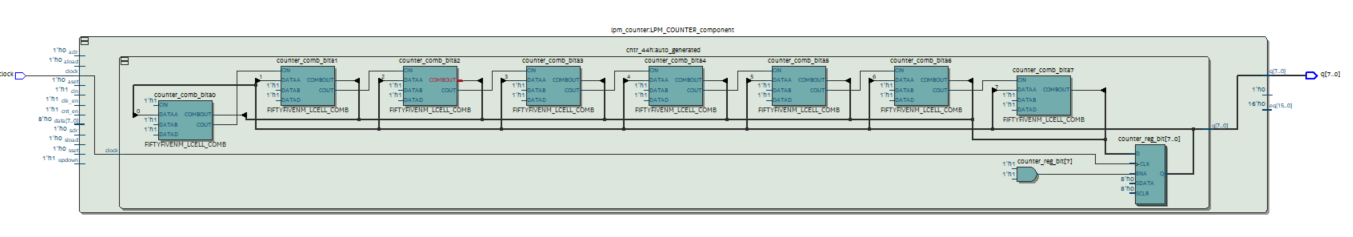
\includegraphics[width=\linewidth]{images/z1_rtl}
		\caption{RTL-схема для обычного счетчика}
		\label{fig:z1_rtl}
	\end{figure}

	\begin{figure}[H]
		\centering
		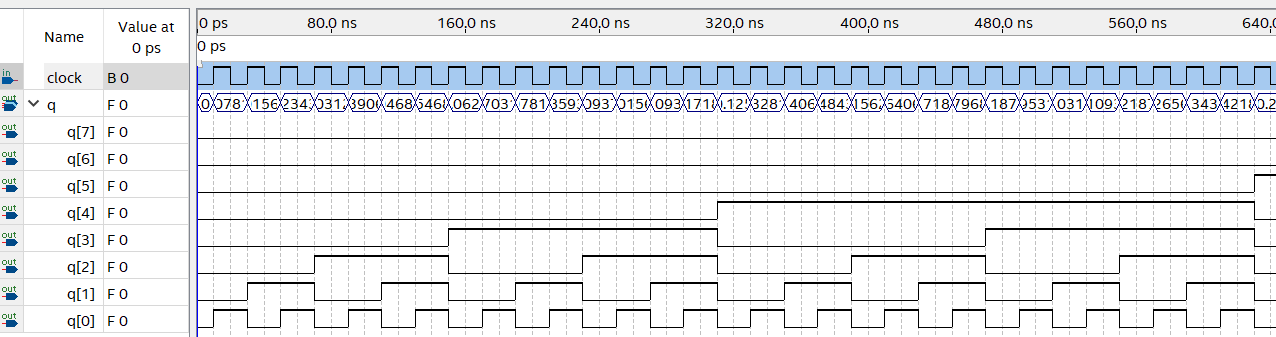
\includegraphics[width=\linewidth]{images/z1_test}
		\caption{Результат тестирования обычного счетчика}
		\label{fig:z1_test}
	\end{figure}

	Был разработан счетчик такой же размерности с возможностью подсчета в положительную и отрицательную сторону, в зависимости от сигнала.
	Результат моделирования на рис. \ref{fig:z2_rtl}. Результат тестирования на рис. \ref{fig:z2_test}.
	
	\begin{figure}[H]
		\centering
		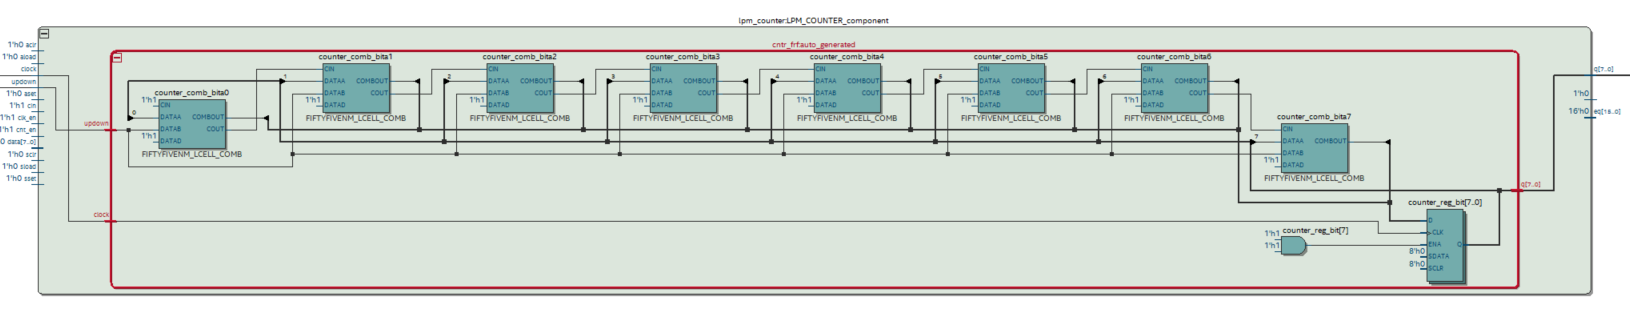
\includegraphics[width=\linewidth]{images/z2_rtl}
		\caption{RTL-схема для счетчика с направлением подсчета}
		\label{fig:z2_rtl}
	\end{figure}
	
	\begin{figure}[H]
		\centering
		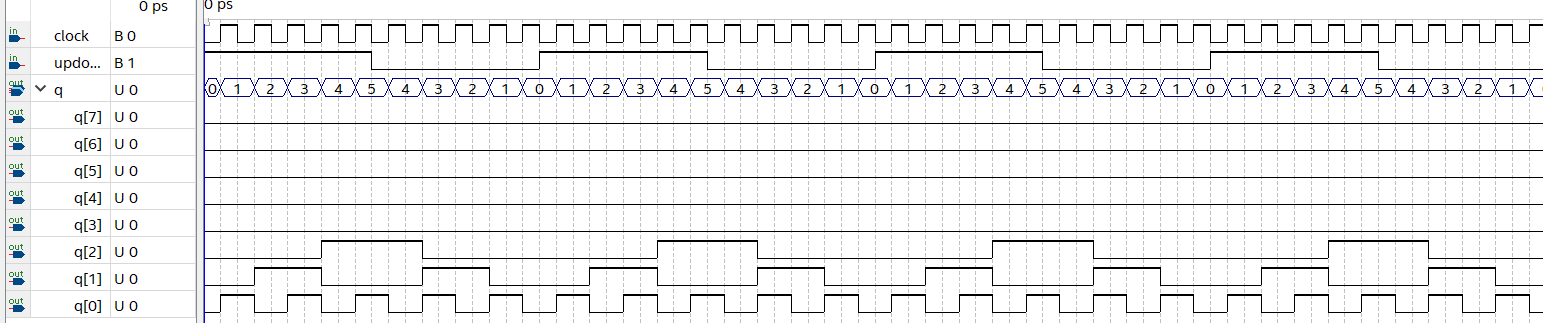
\includegraphics[width=\linewidth]{images/z2_test}
		\caption{Результат тестирования для счетчика с направлением подсчета}
		\label{fig:z2_test}
	\end{figure}

	\subsection{Задание 2}
	
	Исходный код модуля понижал частоту в $2^{24} = 16777216$ раз.
	Такое изменение трудно заметить на симуляции, поэтому код модуля был изменен для понижения частоты в $2^8 = 256$ раз.
	
	Исходный код модуля.
	
	\VerbatimInput{../z1/clk_divider.v}
	
	В оригинальном модуле коэффициент заполнения был равен 50\%.
	Действительно, выходной сигнал был активен в половине случаев.
	Для понижения коэффициента заполнения до 20\% было вычислено значение, начиная с которого необходимо выводить высокий уровень сигнала.
	Результат симуляции на рис. \ref{fig:z3}.
	
	\begin{figure}[H]
		\centering
		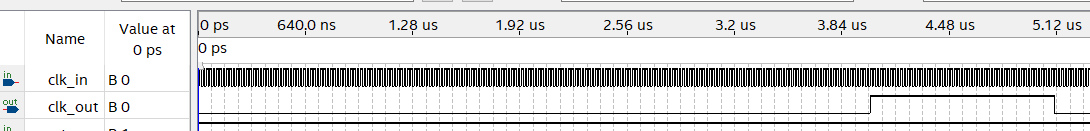
\includegraphics[width=\linewidth]{images/z3}
		\caption{Результат тестирования понижателя частоты}
		\label{fig:z3}
	\end{figure}

	\subsection{Задание 3}

	Чем больше коэффициент заполнения на сигнале ШИМ, тем ярче горит светодиод.
	Пример тестирования представлен на рис. \ref{fig:z4}.
	В результате тестирования яркость светодиода будет постепенно возрастать.
	
	\begin{figure}[H]
		\centering
		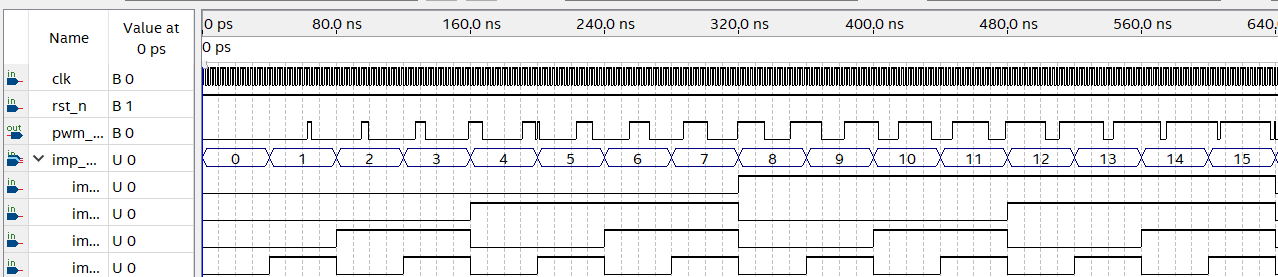
\includegraphics[width=\linewidth]{images/z4}
		\caption{Результат тестирования ШИМ}
		\label{fig:z4}
	\end{figure}

	\subsection{Задание 4}
	
	Был разработан счетчик Грея.
	При положительном фронте $clk$ происходит увеличение счетчика на 1 в коде Грея При этом сигнал $enable$ должен быть 1, в противном случае состояние счетчика не изменится. При подаче сигнала $rst\_n$ равного 0 происходит обнуление счетчика.
	Результат моделирования на рис. \ref{fig:z5_rtl}. Результат тестирования на рис. \ref{fig:z5_test}.
	
	\begin{figure}[H]
		\centering
		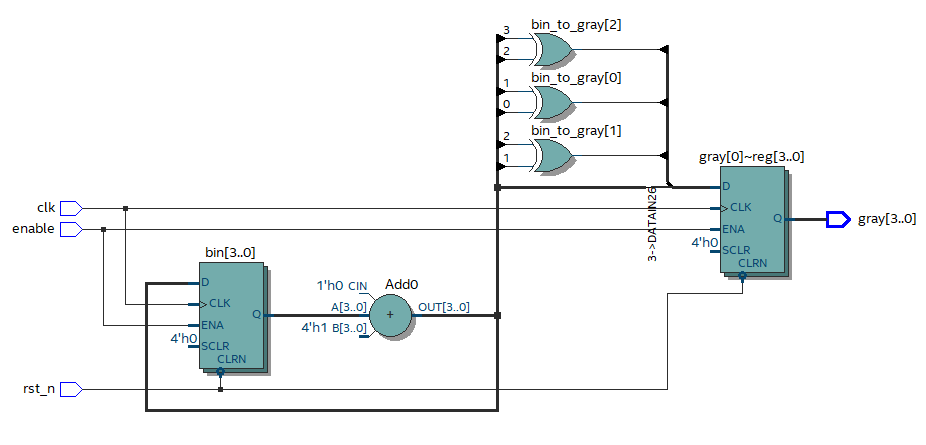
\includegraphics[width=\linewidth]{images/z5_rtl}
		\caption{RTL-схема для счетчика Грея}
		\label{fig:z5_rtl}
	\end{figure}
	
	\begin{figure}[H]
		\centering
		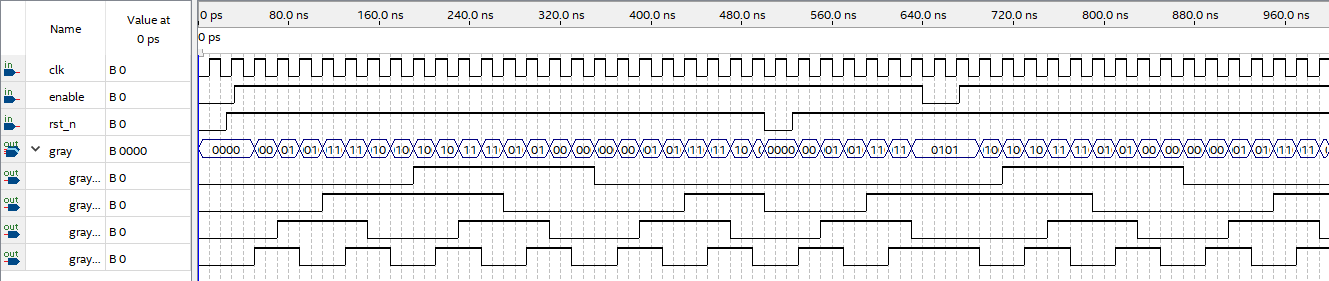
\includegraphics[width=\linewidth]{images/z5_test}
		\caption{Результат тестирования для счетчика Грея}
		\label{fig:z5_test}
	\end{figure}

	\subsection{Задание 5}
	
	Был разработан сдвиговый регистр.
	При подаче сигнала загрузки в регистр загружаются данные.
	Со временем данные смещаются относительно входа в сторону выхода, затем попадают на выход регистра.
	Результат моделирования на рис. \ref{fig:z6_rtl}. Результат тестирования на рис. \ref{fig:z6_test}.
	
	\begin{figure}[H]
		\centering
		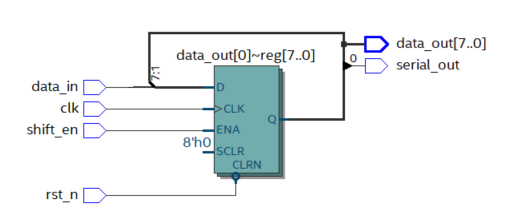
\includegraphics[width=\linewidth]{images/z6_rtl}
		\caption{RTL-схема для сдвигового регистра}
		\label{fig:z6_rtl}
	\end{figure}
	
	\begin{figure}[H]
		\centering
		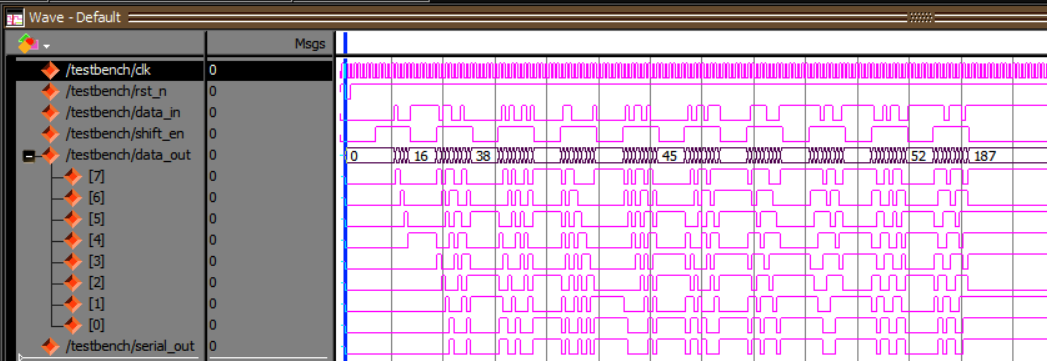
\includegraphics[width=\linewidth]{images/z6_test}
		\caption{Результат тестирования для сдвигового регистра}
		\label{fig:z6_test}
	\end{figure}
	
	
	\section{Задания для самостоятельной работы}
	
	В качестве основы для выполнения задач необходимо использовать проекты из
	Разделов 6.5.1 и 6.6.1. Для демонстрации значений счетчика и сдвигового регистра
	используйте семисегментный дисплей и светодиоды, которые расположены на отладочной
	плате с ПЛИС.
	
	Измените проект счетчика так, чтобы цифры двух произвольных разрядов
	инкрементировались, а цифры других разрядов декрементировались.
			
	Исходный код модуля и результат симуляции на рис. \ref{fig:dop_test}.
	
	\VerbatimInput{../z1/try_dop.v}
	
	\begin{figure}[H]
		\centering
		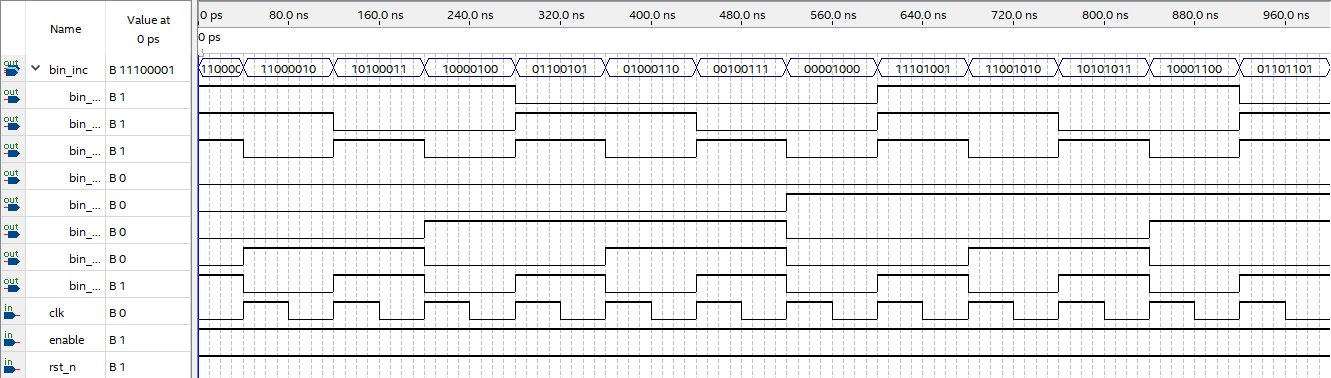
\includegraphics[width=\linewidth]{images/dop_test}
		\caption{Результат тестирования счетчика}
		\label{fig:dop_test}
	\end{figure}
	\section{Контрольные вопросы}
	
	\begin{enumerate}
		\item В чем основные отличия последовательностных устройств от комбинационных?
		
		\item Почему сложно разрабатывать асинхронные схемы, а в современной электронике
		большие асинхронные цифровые схемы практически не используются?
		
		\item Опишите модель Хаффмана для последовательностных устройств .
		
		\item Каково различие между блокирующим и неблокирующим присвоением?
		
		\item К чему приведет изменение порядка операций в блоке always?
		
		\item В каких случаях следует использовать блокирующее присвоение, а в каких - неблокирующее?
		
		\item Опишите порядок выполнения циклов симуляции, определенный в IEEE Verilog	Standart?
		
		\item В результате чего при синтезе возникают защелки (latch), и чем они опасны?
		
		\item Для чего нужны счетчики? Какими они бывают? Опишите на Verilog пример простого
		счетчика.
		
		\item Для каких задач используются делители частоты?
			
		\item Опишите, что такое широтно-импульсная модуляция (ШИМ), и для чего она
		применяется.
		
		\item Как строится счетчик Грея? В чем его особенность? Опишите пример счетчика Грея на
		Verilog.
		
		\item Для чего нужны сдвиговые регистры . Какими бывают виды сдвиговых регистров?
		Приведите пример сдвигового регистра на Verilog.
		
		\item Что такое циклический избыточный код (CRC)? Приведите области применения .
		
		\item Приведите примеры периферийных устройств, используемых с отладочными платами
		ПЛИС; опишите процесс их подключения.
	\end{enumerate}
	
	\section{Выводы по работе}
	
	В ходе работы получен опыт проектирования схем в программе Quartus с помощью языка Verilog.
	Полученное устройство было протестировано с помощью бенчтестов в программе Quartus Simulation Waveform editor и ModelSim.
	В процессе работы были смоделированы счетчики, сдвиговые регистры, ШИМ и счетчик Грея.
	%В процессе работы были смоделированы различные шифраторы и дешифраторы, протестированы способы оптимизации схемы, а так же рассчитаны временные параметры схемы с различными способами оптимизации.
	В процессе был получен опыт работы с платой DE10-Lite, на которой проверялась работоспособность полученного устройства.
	
	\newpage 
	\renewcommand{\refname}{{\normalsize Список использованных источников}} 
	\centering 
	\begin{thebibliography}{9} 
		\addcontentsline{toc}{section}{\refname} 
		\bibitem{Verilog} Thomas D., Moorby P. The Verilog Hardware Description Language. – Springer Science \& Business Media, 2008.
		\bibitem{citekey} Khor W. Y. et al. Evaluation of FPGA Based QSPI Flash Access Using Partial Reconfiguration //2019 7th International Conference on Smart Computing \& Communications (ICSCC). – IEEE, 2019. – С. 1-5
	\end{thebibliography}
	
\end{document} % конец документа
